\documentclass[11pt]{article}
\usepackage{enumitem}
\usepackage{float}
\usepackage[margin=1in]{geometry}
\usepackage{graphicx}
\usepackage[space]{grffile}
\usepackage{adjustbox}
\usepackage{amsmath}
\usepackage{amsthm}
\usepackage{amssymb}
\usepackage{fullpage}
\usepackage{fancyhdr}
\usepackage{xparse}
\usepackage[makeroom]{cancel}
\newcommand{\cnum}{CM146}
\newcommand{\ced}{Fall 2018}
\newcommand{\ctitle}[3]{\title{\vspace{-0.5in}\cnum, \ced\\Problem Set #1: #2}}
\usepackage[usenames,dvipsnames,svgnames,table,hyperref]{xcolor}
\usepackage{listings}
\usepackage{color} %red, green, blue, yellow, cyan, magenta, black, white
\definecolor{mygreen}{RGB}{28,172,0} % color values Red, Green, Blue
\definecolor{mylilas}{RGB}{170,55,241}

\renewcommand*{\theenumi}{\alph{enumi}}
\renewcommand*\labelenumi{(\theenumi)}
\renewcommand*{\theenumii}{\roman{enumii}}
\renewcommand*\labelenumii{\theenumii.}

\author{Zheng Wang (404855295)}
\date{\today}
\title{MATH 151B Homework 5}

\begin{document}

\lstset{language=Matlab,%
	basicstyle=\footnotesize,
	breaklines=true,%
	morekeywords={matlab2tikz},
	keywordstyle=\color{blue},%
	morekeywords=[2]{1}, keywordstyle=[2]{\color{black}},
	identifierstyle=\color{black},%
	stringstyle=\color{mylilas},
	commentstyle=\color{mygreen},%
	showstringspaces=false,%without this there will be a symbol in the places where there is a space
	numbers=left,%
	numberstyle={\tiny \color{black}},% size of the numbers
	numbersep=9pt, % this defines how far the numbers are from the text
	emph=[1]{for,end,break},emphstyle=[1]\color{red}, %some words to emphasise
	%emph=[2]{word1,word2}, emphstyle=[2]{style},
}

\maketitle
\section*{Question 1}
We will first discuss the region of absolute stability for \textbf{Euler's Method}. In Euler's Method, we have the following equation.
\[ \begin{cases}
w_0 = \alpha\\
w_{i+1} = w_i + h\cdot f(t_i, w_i)
\end{cases} \]
Thus, to solve the test equation $ y' = \lambda y, \quad y(0) = \alpha, \quad \text{where $ \lambda < 0 $ } $, we have the following equation\\
\begin{align*}
	w_{i+1} = w_i \cdot Q(\lambda h) &= w_i + h\cdot \lambda w_i\\
	&= w_i\cdot (1 + h\lambda)\\
\end{align*}
Therefore, we have $ Q(\lambda h) = 1+ \lambda h $. Then the following stability region (shown in blue) is obtianed.

\begin{figure}[H]
\centering
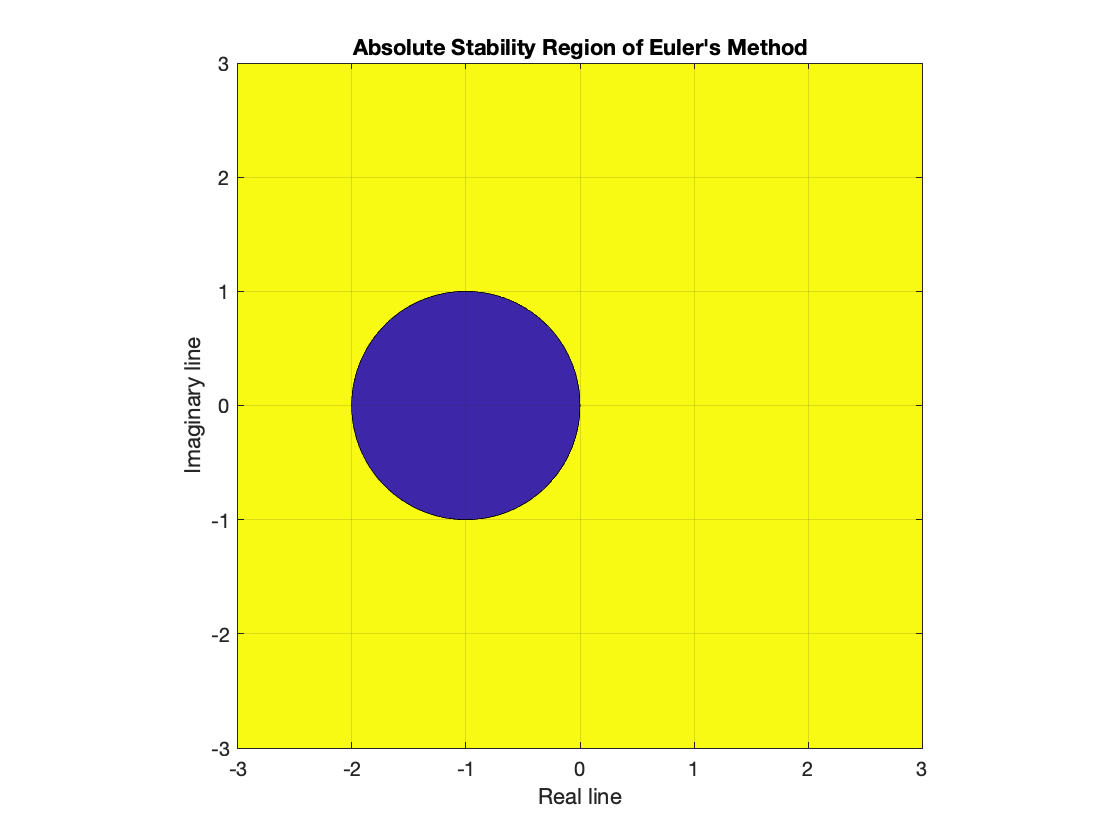
\includegraphics[width = 0.8\linewidth]{abs_eul.png}
\end{figure}\pagebreak
Then, for the \textbf{Midpoint Method}, we have the following equation
\[ \begin{cases}
w_0 = \alpha\\
w_{i+1} = w_i + h\cdot f(t_i + \frac{h}{2}, w_i + \frac{h}{2} f(t_i,w_i))
\end{cases} \]
Therefore, we have the following when solving the test equation:
\begin{align*}
	w_{i+1} &= w_i + h\cdot \left( \lambda \left( w_i + \frac{h}{2} \lambda w_i \right) \right)\\
	&= w_i \cdot \left( 1 + h\lambda + \frac{\lambda^2 h^2}{2} \right)
\end{align*}
Therefore, we have $ \displaystyle Q(\lambda h) = 1 + \lambda h + \frac{\lambda^2 h^2}{2} $. Then we generate the following absolute stability region (colored blue):

\begin{figure}[H]
\centering
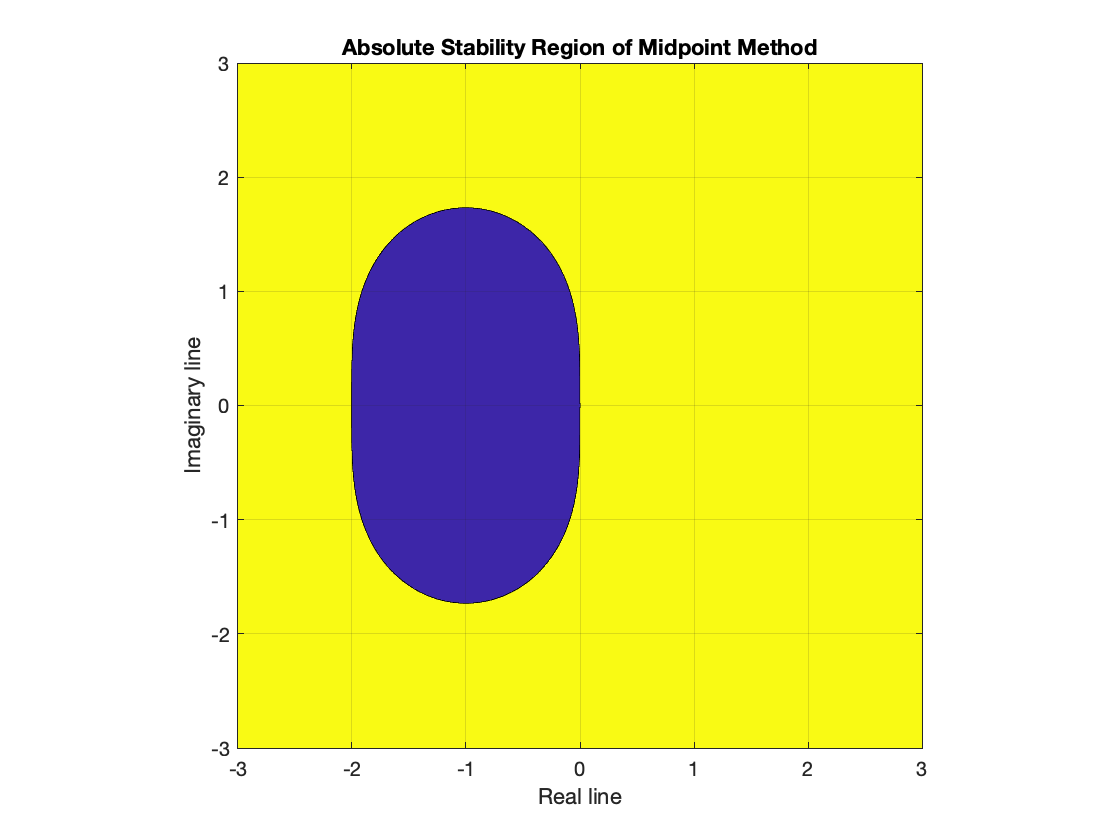
\includegraphics[width = 0.8\linewidth]{abs_mid.png}
\end{figure}
The code to generate the above plots are given below:
\lstinputlisting{q1.m}\pagebreak

\section*{Question 2}
We will first derive the equation of estimating $ y_0' $. Suppose that $x_0 = 0$ and $x_i = x_0 + ih = ih $. Then, by Lagrange interpolation, we have
\begin{align*}
	 y(x) &= y(x_0)\cdot\frac{(x-x_1)(x-x_2)}{(x_0 - x_1)(x_0-x_2)} + y(x_1) \cdot \frac{(x-x_0)(x-x_2)}{(x_1 - x_0)(x_1-x_2)}\\
	 &+  y(x_2) \cdot \frac{(x-x_0)(x-x_1)}{(x_2 - x_0)(x_2-x_1)} + \frac{(x-x_0)(x-x_1)(x-x_2)}{6}f'''(\xi(x))
\end{align*}
Therefore, by taking the derivative and evaluate at $x_0$, we have the following
\begin{align*}
	y'(x_0) &= y(x_0)\left[ \frac{2x_0 - x_1 - x_2}{(x_0 - x_1)(x_0-x_2)} \right] + y(x_1) \left[ \frac{2x_0 - x_0 - x_2}{(x_1 - x_0)(x_1-x_2)} \right] \\
	&+ y(x_2)\left[ \frac{2x_0 - x_0 - x_1}{(x_2 - x_0)(x_2-x_1)} \right] + \frac{1}{6}f'''(\xi_0) (x_0-x_1)(x_0-x_2)\\
	&= - \frac{3}{2h}w_0 + \frac{2}{h}w_1 - \frac{1}{2h}w_2 + \frac{h^2}{3}f'''(\xi_0) \qquad \text{where $\xi_0 \in (0,h)$}
\end{align*}
Thus, the estimate of $ y'(0) $ has accuracy of $\mathcal{O}(h^2)$, and by truncating the $f'''(\xi_0)$ term, we then obtain the following equation of $w_0$, $w_1$, and $w_2$:
\[ 0 = 2h \cdot y'(0) = -3w_0 + 4w_1 - w_2 \]
 Next, since the BVP has the form $y'' = p(x)y' + q(x)y + r(x) $, by using the cenrtal-finite-difference formula, we obtian the following for $ w_i $, where $ i = 1, 2, ..., N-1 $:
 \[ -\left(1+\frac{h}{2}p(x_i)\right)w_{i-1} + (2+h^2q(x_i))w_i -\left(1-\frac{h}{2}p(x_i)\right)w_{i+1} = -h^2r(x_i) \]
 For the BVP we are solving, as $p(x) = 0$, $q(x) = 4$, and $r(x) = -4x$; we simplify the above equation to the following:
 \[ w_{i-1} - (2+4h^2)w_i + w_{i+1} = -4h^2\cdot x_i \]
Finally, as the last equation is $w_N = 1$, we can write the system in the matrix form $A\vec{w} = \vec{b}$, where
 \[A = \begin{bmatrix}
 	-3 & 4  & -1 & 0 &  \dots & 0\\
	1 & -(2+4h^2) & 1 & 0 & \dots & 0 \\
	0 & 1 & -(2+4h^2) & 1 & \dots & 0 \\
	\vdots & \ddots &  \ddots & \ddots & \ddots & \vdots \\
	\vdots &  & \ddots & \ddots & \ddots & 1 \\
	0 & \dots & \dots & 0 & 1 & -(2+4h^2)
\end{bmatrix} \]
\[ \vec{w} = \begin{bmatrix}
	w_0\\
	w_1\\
	\vdots\\
	w_{N-2}\\
	w_{N-1}
\end{bmatrix}\qquad \text{and}\qquad
\vec{b} = \begin{bmatrix}
	0\\
	-4h^2x_1\\
	\vdots\\
	-4h^2x_{N-2}\\
	-4h^2x_{N-1} - 1
\end{bmatrix} \qquad \text{(Note: $w_N = 1$ from question)}\]\pagebreak\\
\textbf{Then we can generate the solution to the BVP with the following code:}\\
\lstinputlisting{q2.m}

\textbf{The plot obtained from the code above is:}\\
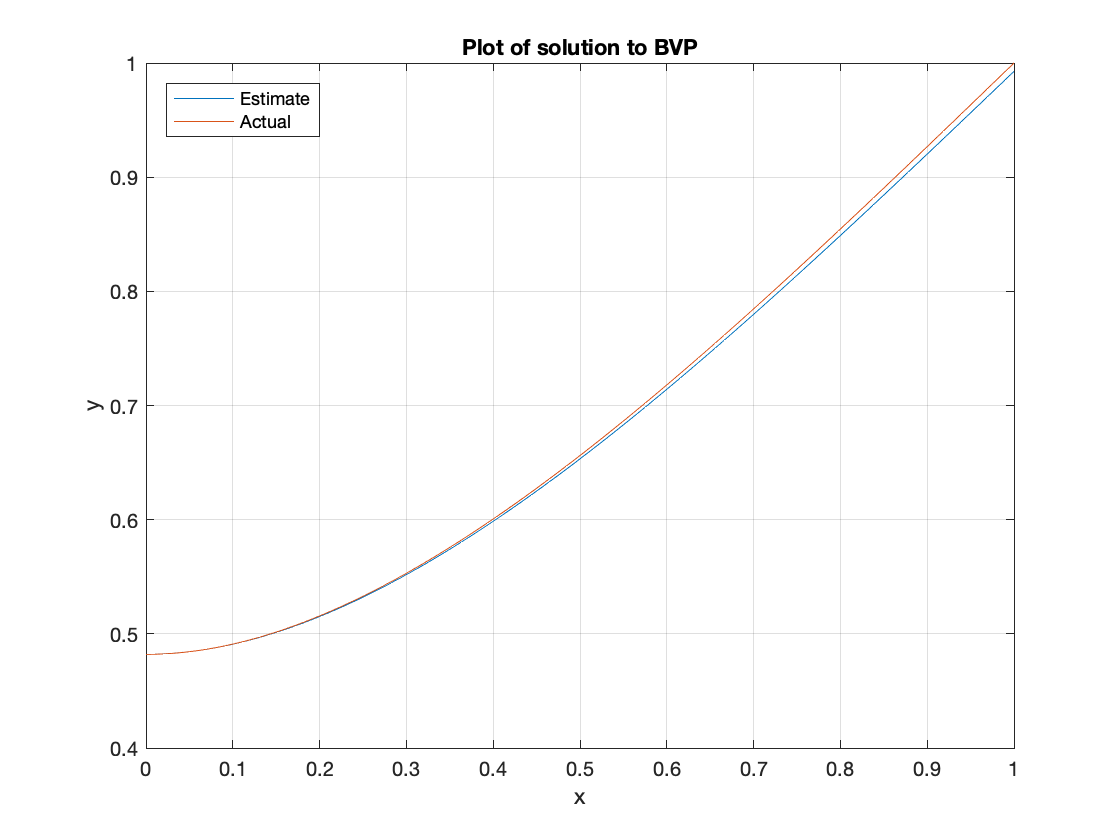
\includegraphics[width=\linewidth]{plot_y.png}\\\\

\textbf{The estimate of $y(0)$ is $\boxed{0.4821}$. The console will output the following:}
\begin{verbatim}
    >> q2
        0.4821
\end{verbatim}


\end{document}
